%%%%%%%%%%%%%%%%%%%%%%%%%%%%%%%%%%%%%%%%%%%%%%%%%%%%%%%%%%%%%%%
%
% Welcome to Overleaf --- just edit your LaTeX on the left,
% and we'll compile it for you on the right. If you open the
% 'Share' menu, you can invite other users to edit at the same
% time. See www.overleaf.com/learn for more info. Enjoy!
%
%%%%%%%%%%%%%%%%%%%%%%%%%%%%%%%%%%%%%%%%%%%%%%%%%%%%%%%%%%%%%%%

% Inbuilt themes in beamer
\documentclass{beamer}

% Theme choice:
\usetheme{CambridgeUS}
\usepackage{amsmath}
\providecommand{\pr}[1]{\ensuremath{\Pr\left(#1\right)}}
\providecommand{\cdf}[2]{\ensuremath{\text{F}_{#1}\left(#2\right)}}

% Title page details: 
\title{Assignment 9} 
\author{Gautam Singh (CS21BTECH11018)}
\date{\today}
\logo{\large \LaTeX{}}


\begin{document}

% Title page frame
\begin{frame}
    \titlepage 
\end{frame}

% Remove logo from the next slides
\logo{}


% Outline frame
\begin{frame}{Outline}
    \tableofcontents
\end{frame}


% Lists frame
\section{Problem}
\begin{frame}{Problem Statement}

\textbf{(NCERT Class 12, Exercise 13.5.3 )} There are 5\% defective items in a large bulk of items. What is the probability that a sample of 10 items will include not more than one defective item?

\end{frame}


% Blocks frame
\section{Solution}
\begin{frame}{Solution}
    \begin{block}{Random Variables}
        \begin{enumerate}
        		\item $X_i$: Bernoulli random variables with parameter $p, 1 \leq i \leq N$
        		\item $Y$: Binomial random variable given by $Y = \sum_{i = 1}^{i = N}X_i$
        \end{enumerate}
    \end{block}
    \begin{exampleblock}{Moment Generating Function of $X_i$ and $Y$}
		\begin{align}
			M_Z(X_i) &= \sum_{k = -\infty}^{k = \infty}z^{-k}P_X(k) \\
			&= P_X(0) + z^{-1}P_X(1) = (1 - p) + pz^{-1} \\
			\label{mgf-X}
		\end{align}
    \end{exampleblock}
\end{frame} 

\begin{frame}
	\begin{exampleblock}{Moment Generating Function of $Y$}
		\begin{align}
			M_Y(Z) &= E(Z^{-Y}) = E(Z^{-\sum_{i = 1}^{i = N}X_i}) \\
			&= \prod_{i = 1}^{i = N}E(Z^{-X_i}) \\		
			&= [(1 - p) + pz^{-1}]^N \\
			&= \sum_{k = 0}^{k = N}z^{-k}(\binom{N}{k}(1 - p)^{N - k}p^k)
			\label{mgf-Y}		
		\end{align}
	\end{exampleblock}
	\begin{alertblock}{PMF of Y}
		\begin{align}
			\pr{Y = k} = 
			\begin{cases}
			\binom{N}{k}(1 - p)^{N - k}p^k, & 0 \leq k \leq N \\
			0, & \textrm{otherwise}
			\end{cases}
			\label{pmf-Y}		
		\end{align}
	\end{alertblock}
\end{frame}

\begin{frame}
	\begin{alertblock}{CDF of Y}
		\begin{align}
			\cdf{Y}{k} = \sum_{i = -\infty}^{i = k}\pr{Y = i} =
			\begin{cases}
			0, & k < 0 \\
			\sum_{K = 0}^{K = k}\binom{N}{K}(1 - p)^{N - K}p^K, & 0 \leq k < N \\
			1, & k \geq N
			\end{cases}
			\label{cdf-Y}		
		\end{align}
	\end{alertblock}
	\begin{alertblock}{Problem parameters}
		Given:
    		\begin{enumerate}
    			\item $p$ = 0.05
    			\item $N$ = 10
    		\end{enumerate}
		To find: $F_Y(1)$    
    \end{alertblock}
\end{frame}

\begin{frame}{Graphs for PMF and CDF}
	\begin{figure}
		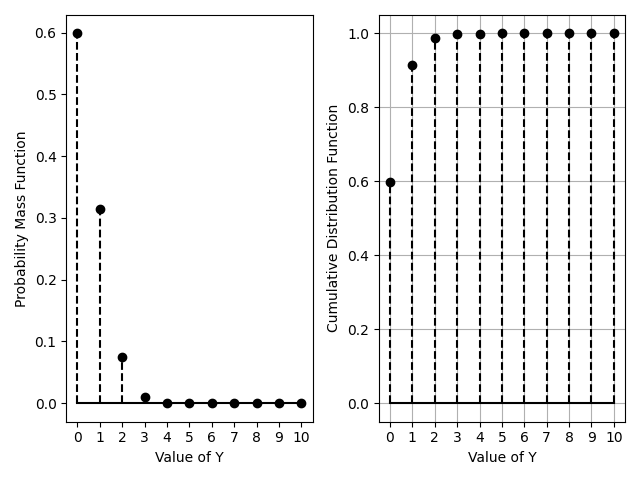
\includegraphics[height=0.7\textheight, width=0.7\textwidth, keepaspectratio]{figs/9_1.png}
		\caption{Graphs of PMF and CDF of Binomial Random Variable Y}
		\label{fig:pmf-cdf}
	\end{figure}
\end{frame}

\begin{frame}{Solution}
	\begin{align}
		\cdf{Y}{1} &= \sum_{i = 0}^{i = 1}\binom{10}{i}(1 - 0.05)^{10 - i}(0.05)^i \\
		&= (0.95)^{10} + 10(0.95)^9(0.05) = 0.914
	\end{align}
\end{frame}

\end{document}